\documentclass[a4paper,12pt, french]{report}

\usepackage{fancyhdr}

% Utilisation de tous les packages nécéssaires
\usepackage[a4paper, total={7in, 10in}]{geometry}
\usepackage[utf8]{inputenc}
\usepackage[utf8]{inputenc}%           gestion des accents (source)
\usepackage[T1]{fontenc}%              gestion des accents (PDF)
\usepackage[francais]{babel}%          gestion du français
\usepackage{textcomp}%                 caractères additionnels
\usepackage{lmodern}%                  police de caractère
\usepackage{geometry}%                 gestion des marges
\usepackage{graphicx}%                 gestion des images
\usepackage{array}%                    gestion améliorée des tableaux
\usepackage{calc}%                     syntaxe naturelle pour les calculs
\usepackage{amsmath}
\usepackage{dsfont}
\usepackage{color}
\usepackage{url}
\usepackage{hyperref}
\usepackage{listings} %Algorithmes
\usepackage{listingsutf8}

\definecolor{mygreen}{rgb}{0,0.6,0}
\definecolor{mygray}{rgb}{0.5,0.5,0.5}
\definecolor{mymauve}{rgb}{0.58,0,0.82}

\graphicspath{ {images/} }


\hypersetup{
colorlinks=true, %colorise les liens
breaklinks=true, %permet le retour à la ligne dans les liens trop longs
urlcolor= blue, %couleur des hyperliens
linkcolor= black, %couleur des liens internes
citecolor=blue,    %couleur des liens de citations
}


\definecolor{Comments}{rgb}{0.13,0.54,0.13}
\definecolor{Strings}{rgb}{0,0.63,0}
\definecolor{Keywords}{rgb}{0,0,1}
\definecolor{Background}{rgb}{1,1,1}
\definecolor{Variables}{rgb}{0.62, 0.12, 0.94}

\tolerance=1000

\title{PAO: Développement d'une bibliothèque musicale}
\author{Alexis \bsc{Durieux}}
\date{ASI4 - 2017}

\pagestyle{fancy}
\fancyhead[R]{}
\fancyhead[L]{
\includegraphics[scale=0.35]{insa-logo.png}}

\begin{document}
\maketitle
\tableofcontents

\chapter*{Introduction}
L'objectif de ce PAO est la mise en application des concepts de bases de données par la mise en place d'une petite base de données et de son utilisation pour réaliser un ensemble de fonctionnalités. Dans notre cas, l'objectif est la création d'une bibliothèque musicale permettant à un utilisateur l'enregistrement de sa discographie. A ces fins nous allons réaliser une base de données. Pour concevoir cette dernière au mieux nous allons procéder par étapes. Dans un premier nous allons analyser les besoins de l'applications, puis nous allons réaliser le modèle entité-attribut avant de passer au modèle relationnel. Avec la base de données créée nous allons pouvoir réaliser une application java simple basée sur cette dernière. Nous implémenterons le pattern \textbf{DAO} afin de passer du \emph{modèle relationnel} à un \emph{modèle objet}. En terme de technologie, nous utiliserons une base de données \emph{Postgres} et \emph{JDBC} pour faire le liant avec l'application JAVA afin d'implémenter le pattern \textbf{DAO}

\chapter{Analyse des besoins de l'application}
Nous voulons donc créer une application permettant à l'utilisateur d'enregistrer ses musiques, artistes et albums afin de pouvoir les consulter. L'utilisateur utilise la bibliothèque de l'application pour ajouter ces derniers à sa  bibliothèque personnelle. Néanmoins l'utilisateur peut ajouter directement des musiques, albums et artistes à sa bibliothèque personnelle qui sont donc ajoutés à la bibliothèque de l'application. C'est donc une bibliothèque musicale collaborative que nous cherchons à créer où les données ajoutées par un utilisateur servent à tous les utilisateurs. On suppose également les relations suivantes. Un titre est contenu dans un album et un album est composé par un artiste. Ces relations sont primordiales à la bonne création de nos tables. En plus de vouloir stocker des titres, artistes et albums, on veut également stocker des informations propres à l'utilisateur. Enfin ce dernier doit être en mesure de stocker des écoutes et de créer et modifier des playlists. On suppose qu'une fois créé un titre ne peut être modifié ou supprimé de la bibliothèque de l'application. En effet une modification par un utilisateur engendrera sinon une modification potentielle dans la bibliothèque d'autres utilisateurs.
\chapter{Modèle entité-attribut et relationnel}
\section{Modélisation entité-attribut}
  \includegraphics[scale=0.5]{ea-final.png}
\section{Modélisation de la vue}
  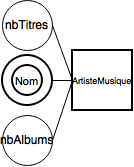
\includegraphics[scale=0.5]{vues.png}
\section{Du modèle entité-attribut vers le modèle relationnel}
  \subsection{Tables, clés primaires et cardinalité}
    \begin{itemize}
      \item Utilisateur(\underline{pseudo}, motDePasse, nom, prenom, age) \newline
        La table \emph{Utilisateur} référence les utilisateurs. On choisit comme \textbf{clé primaire} un \emph{pseudo} en raison des homonymes possibles entre utilisateurs.
      \item Titre(\underline{id}, nom, duree, nomAlbum, genre) \newline
        La table \emph{Titre} référence les titres. On choisit un \textbf{id} \textbf{clé primaire} en raison des homonymies possibles entre \textbf{plusieurs} titres. On a également un \emph{nomAlbum} afin de représenter la cardinalité. En effet on suppose qu'un titre n'appartient au plus qu'à un seul album. Le \emph{genre} quand à lui est un attribut issu d'une énumération définissant une liste de genre de musique.
       \item Album(\underline{nom}, nomArtiste, annee) \newline
        La table \emph{Album} référence les albums. On suppose dans notre cas que deux albums ne peuvent avoir le même nom. On peut donc choisir \textbf{nom} comme \textbf{clé primaire}. La clé étrangère \emph{nomArtiste} représente le fait qu'un album est composé par un seul artiste.
      \item Artiste(\underline{nom}, nationalite) \newline
        La table \emph{Artiste} référence les \emph{artistes}. Ici on a choisit comme \textbf{clé primaire} le \emph{nom} car on suppose que deux artistes ne peuvent pas avoir le même nom.
      \item ListeTitre(\underline{pseudoUser}, \underline{titreId}) \newline
        La table \emph{ListeTitre} correspond aux titres enregistrés par un utilisateur dans sa bibliothèque. On associe un utilisateur à un titre. La \textbf{clé primaire}: est \textbf{(pseudoUser, titreId)} car un utilisateur ne peut enregistrer deux titres identiques dans sa bibliothèque. En revanche un titre peut être enregistré dans la bibliothèque respective de \textbf{plusieurs} utilisateurs.
      \item ListeAlbum(\underline{pseudoUser}, \underline{nomAlbum}) \newline
        La table \emph{ListeAlbum} correspond aux albums enregistrés par un utilisateur dans sa bibliothèque. On associe un utilisateur à un titre. La \textbf{clé primaire}: est \textbf{(pseudoUser, nomAlbum)} car un utilisateur ne peut enregistrer deux albums identiques dans sa bibliothèque. En revanche un album peut être enregistré dans la bibliothèque respective de \textbf{plusieurs} utilisateurs.
      \item ListeArtiste(\underline{pseudoUser}, \underline{nomArtiste}) \newline
        La table \emph{ListeArtiste} correspond aux artistes enregistrés par un utilisateur dans sa bibliothèque. On associe un \textbf{utilisateur} à un \textbf{titre}. La \textbf{clé primaire}: est \textbf{(pseudoUser, nomArtiste)} car un utilisateur ne peut enregistrer deux artistes identiques dans sa bibliothèque. En revanche un artiste peut être enregistré dans la bibliothèque respective de \textbf{plusieurs} utilisateurs.
      \item Ecoute(\underline{pseudoUser}, \underline{date}, idTitre) \newline
        La table \emph{Ecoute} correspond à une liste d'écoute. À un instant \emph{t}, un utilisateur écoute un titre. On les associe donc dans la table. On choisit comme \textbf{clé primaire}: \textbf{(pseudoUser, date)}. En effet, un utilisateur ne peut écouter deux musiques en même temps.
      \item Playlist(\underline{id}, pseudoUser, nom) \newline
        La table \emph{Playlist} référence les playlists des utilisateurs. La \textbf{clé primaire} est un \emph{id} car un utilisateur peut avoir \textbf{plusieurs} playlists. On ne peut également choisir le \emph{nom} car deux utilisateurs différents peuvent avoir une playlist ayant le même nom. En raison de la table \textbf{PlaylistTitre}, on utilise \textbf{id} comme clé primaire car clé étrangère de \textbf{PlaylistTitre}.
      \item PlaylistTitre(\underline{idTitre}, \underline{idPlaylist}) \newline
        La table \emph{PlaylistTitre} référence les titres des playlists. La \textbf{clé primaire} est \textbf{(idTitre, idPlaylist)} car un titre peut être présent une seule fois dans une même \emph{playlist} mais être présent dans \textbf{plusieurs} playlists différentes.
    \end{itemize}
  \subsection{Vue}
    \begin{itemize}
       \item  La \textbf{vue} \emph{ArtisteMusique} aggrège un \emph{artiste} avec son \emph{nombre de titres} et \emph{nombre d'albums} calculés respectivement à partir des tables \emph{Titre} et \emph{Artiste}.
    \end{itemize}

\section{Contraintes d'intégrité et types}
  \subsection{Définitions des types et tables}
    \begin{itemize}
      \item \underline{GENRE\_MUSIQUE - ÉNUMÉRATION}
        \begin{itemize}
          \item \textbf{pop, rock, jazz, blues, electronique, variété, rap, reggae}
        \end{itemize}
      \item \underline{Utilisateur}
        \begin{itemize}
          \item pseudo: \textbf{VARCHAR(15) PRIMARY KEY}
          \item motDePasse: \textbf{VARCHAR(64) NOT NULL}
          \item nom: \textbf{VARCHAR(15)}
          \item prenom: \textbf{VARCHAR(15)}
          \item age: \textbf{INTEGER} $\in ]0, 99[$
        \end{itemize}
      \item Titre
        \begin{itemize}
          \item id: \textbf{INTEGER PRIMARY KEY}
          \item nom: \textbf{VARCHAR(50) NOT NULL}
          \item duree: \textbf{INTEGER NOT NULL}
          \item nomArtiste: \textbf{VARCHAR(25) FOREIGN KEY REFERENCES ARTISTE NOT NULL}
          \item nomAlbum: \textbf{VARCHAR(25) FOREIGN KEY REFERENCES ALBUM}
          \item genre: \textbf{GENRE\_MUSIQUE}
          Il faut noter qu'on utilise une \textbf{séquence} de \textbf{INTEGER} pour définir la valeur de \textbf{id}
        \end{itemize}
      \item Album
        \begin{itemize}
          \item nom: \textbf{VARCHAR(25) PRIMARY KEY}
          \item nomArtiste: \textbf{VARCHAR(25) REFERENCES ARTISTE NOT NULL}
          \item annee: \textbf{INTEGER} $\in ]0, 3000[$
        \end{itemize}
      \item Artiste
        \begin{itemize}
          \item nom: \textbf{VARCHAR(25) PRIMARY KEY}
          \item nationalite: \textbf{VARCHAR(50)}
        \end{itemize}
      \item ListeTitre
        \begin{itemize}
          \item pseudoUser: \textbf{VARCHAR(15) FOREIGN KEY REFERENCES UTILISATEUR}
          \item titreId: \textbf{INTEGER FOREIGN KEY REFERENCES TITRE}
          \item \textbf{PRIMARY KEY: (pseudoUser, titreId)}
        \end{itemize}
      \item ListeAlbum
        \begin{itemize}
          \item pseudoUser: \textbf{VARCHAR(15) FOREIGN KEY REFERENCES UTILISATEUR}
          \item nomAlbum: \textbf{VARCHAR(25) FOREIGN KEY REFERENCES ALBUM}
          \item \textbf{PRIMARY KEY: (pseudoUser, nomAlbum)}
        \end{itemize}
      \item ListeArtiste
        \begin{itemize}
          \item pseudoUser: \textbf{VARCHAR(15) FOREIGN KEY REFERENCES UTILISATEUR}
          \item nomArtiste: \textbf{VARCHAR(25) FOREIGN KEY REFERENCES ARTISTE}
          \item \textbf{PRIMARY KEY: (pseudoUser, nomArtiste)}
        \end{itemize}
      \item Ecoute
        \begin{itemize}
          \item pseudoUser: \textbf{VARCHAR(15) FOREIGN KEY REFERENCES UTILISATEUR}
          \item dateEcoute: \textbf{TIMESTAMP DEFAULT CURRENT\_TIMESTAMP}
          \item titreId: \textbf{INTEGER FOREIGN KEY REFERENCES TITRE}
          \item \textbf{PRIMARY KEY: (pseudoUser, dateEcoute)}
        \end{itemize}
      \item Playlist
        \begin{itemize}
          \item id: \textbf{VARCHAR(10) PRIMARY KEY}
          \item nom: \textbf{VARCHAR(25) NOT NULL}
          \item pseudoUser: \textbf{VARCHAR(15) FOREIGN KEY REFERENCES UTILISATEUR}
          Il faut noter qu'on utilise une \textbf{séquence} de \textbf{INTEGER} pour définir la valeur de \textbf{id}
        \end{itemize}
      \item PlaylistTitre
        \begin{itemize}
          \item titreId: \textbf{INTEGER FOREIGN KEY REFERENCES TITRE}
          \item playlistId: \textbf{INTEGER FOREIGN KEY REFERENCES PLAYLIST}
          \item \textbf{PRIMARY KEY: (titreId, playlistId)}
        \end{itemize}
      \end{itemize}
  \subsection{Définitions des triggers }
    \begin{itemize}
      \item Suppression dans \textbf{PLAYLIST} \newline
        Une suppression d'une playlist dans la table \textbf{PLAYLIST}, engendre la suppression de toutes les références associées dans la table \textbf{'PLAYLIST\_TITRE'}.
    \end{itemize}

\chapter{Développement d'une application JAVA}
\section{Cahier des charges}
  \subsection{Présentation du principe de l'application}
    La bibliothèque musicale que l'on souhaite développer est une bibliothèque musicale inspirée des plateformes populaires existantes (Spotify, Deezer)...À Contrario de ces dernières, cette application ne permettra pas d'écouter directement des titres mais permettra néanmoins d'enregistrer les écoutes récentes. Néanmoins, cette application permettra à l'utilisateur de classifier sa musique, de la trier et potentiellement dans un dernier de se voir recommander des musiques.
  \subsection{Cas d'utilisations et fonctionnalités}
    Les spécifications que nous allons lister ci-après sont l'ensemble des fonctionnalités permisent à l'utilisateur de l'application:
    \begin{itemize}
      \item Un utilisateur peut créer un compte auquel il pourra se connecter à l'aide d'un pseudonyme et d'un mot de passe.
      \item La connexion au compte est nécessaire pour accéder à l'application. \newline
        \textbf{Nous supposerons maintenant que l'utilisateur est connecté pour les fonctionnalités suivantes}
      \item L'utilisateur peut ajouter manuellement des titres à la bibliothèque de l'application.
      \item L'utilisateur peut ajouter manuellement des artistes à la bibliothèque de l'application.
      \item L'utilisateur peut ajouter manuellement des albums à la bibliothèque de l'application.
      \item L'utilisateur peut ajouter des titres à sa bibliothèque personnelle\footnote{Contenu visible seulement par l'utilisateur}.
      \item L'utilisateur peut ajouter des artistes à sa bibliothèque personnelle.
      \item L'utilisateur peut ajouter des albums à sa bibliothèque personnelle.
      \item L'utilisateur peut créer des playlists à partir des titres de la bibliothèque de l'application.
      \item L'utilisateur peut enregistrer ses écoutes récentes.
      \item L'utilisateur peut retirer des écoutes récentes.
      \item L'utilisateur peut voir des recommandations basées sur ses écoutes récentes
      \item L'utilisateur peut rechercher des titres, artistes, albums.
    \end{itemize}
  \subsection{Modèle DAO et Diagramme de classe}
    Dans le cadre de ce projet nous utiliserons le \textbf{Design Pattern DAO (Data Access Object)}. Ce \textbf{Design pattern} permet de séparer l'accès aux bases de données à l'utilisation même de ces données au sein de l'application. Ainsi cela va consister dans notre cas à créer des classes correspondant aux entités que l'on compte manipuler dans notre application dans un premier temps. Seulement au lieu de faire ces classes manipuler directement la base de données, nous allons utiliser des classes \textbf{DAO} s'occupant de l'accès à la base de données pour l'entité correspondante. Par exemple \textbf{TitreDAO} va contenir les opérations relative à la classe \textbf{Titre} en base de données. Ce pattern \textbf{DAO} nous permet de passer d'un \textbf{modèle relationnel à un modèle objet}. On obtient donc le diagramme de classe ci-dessous:
    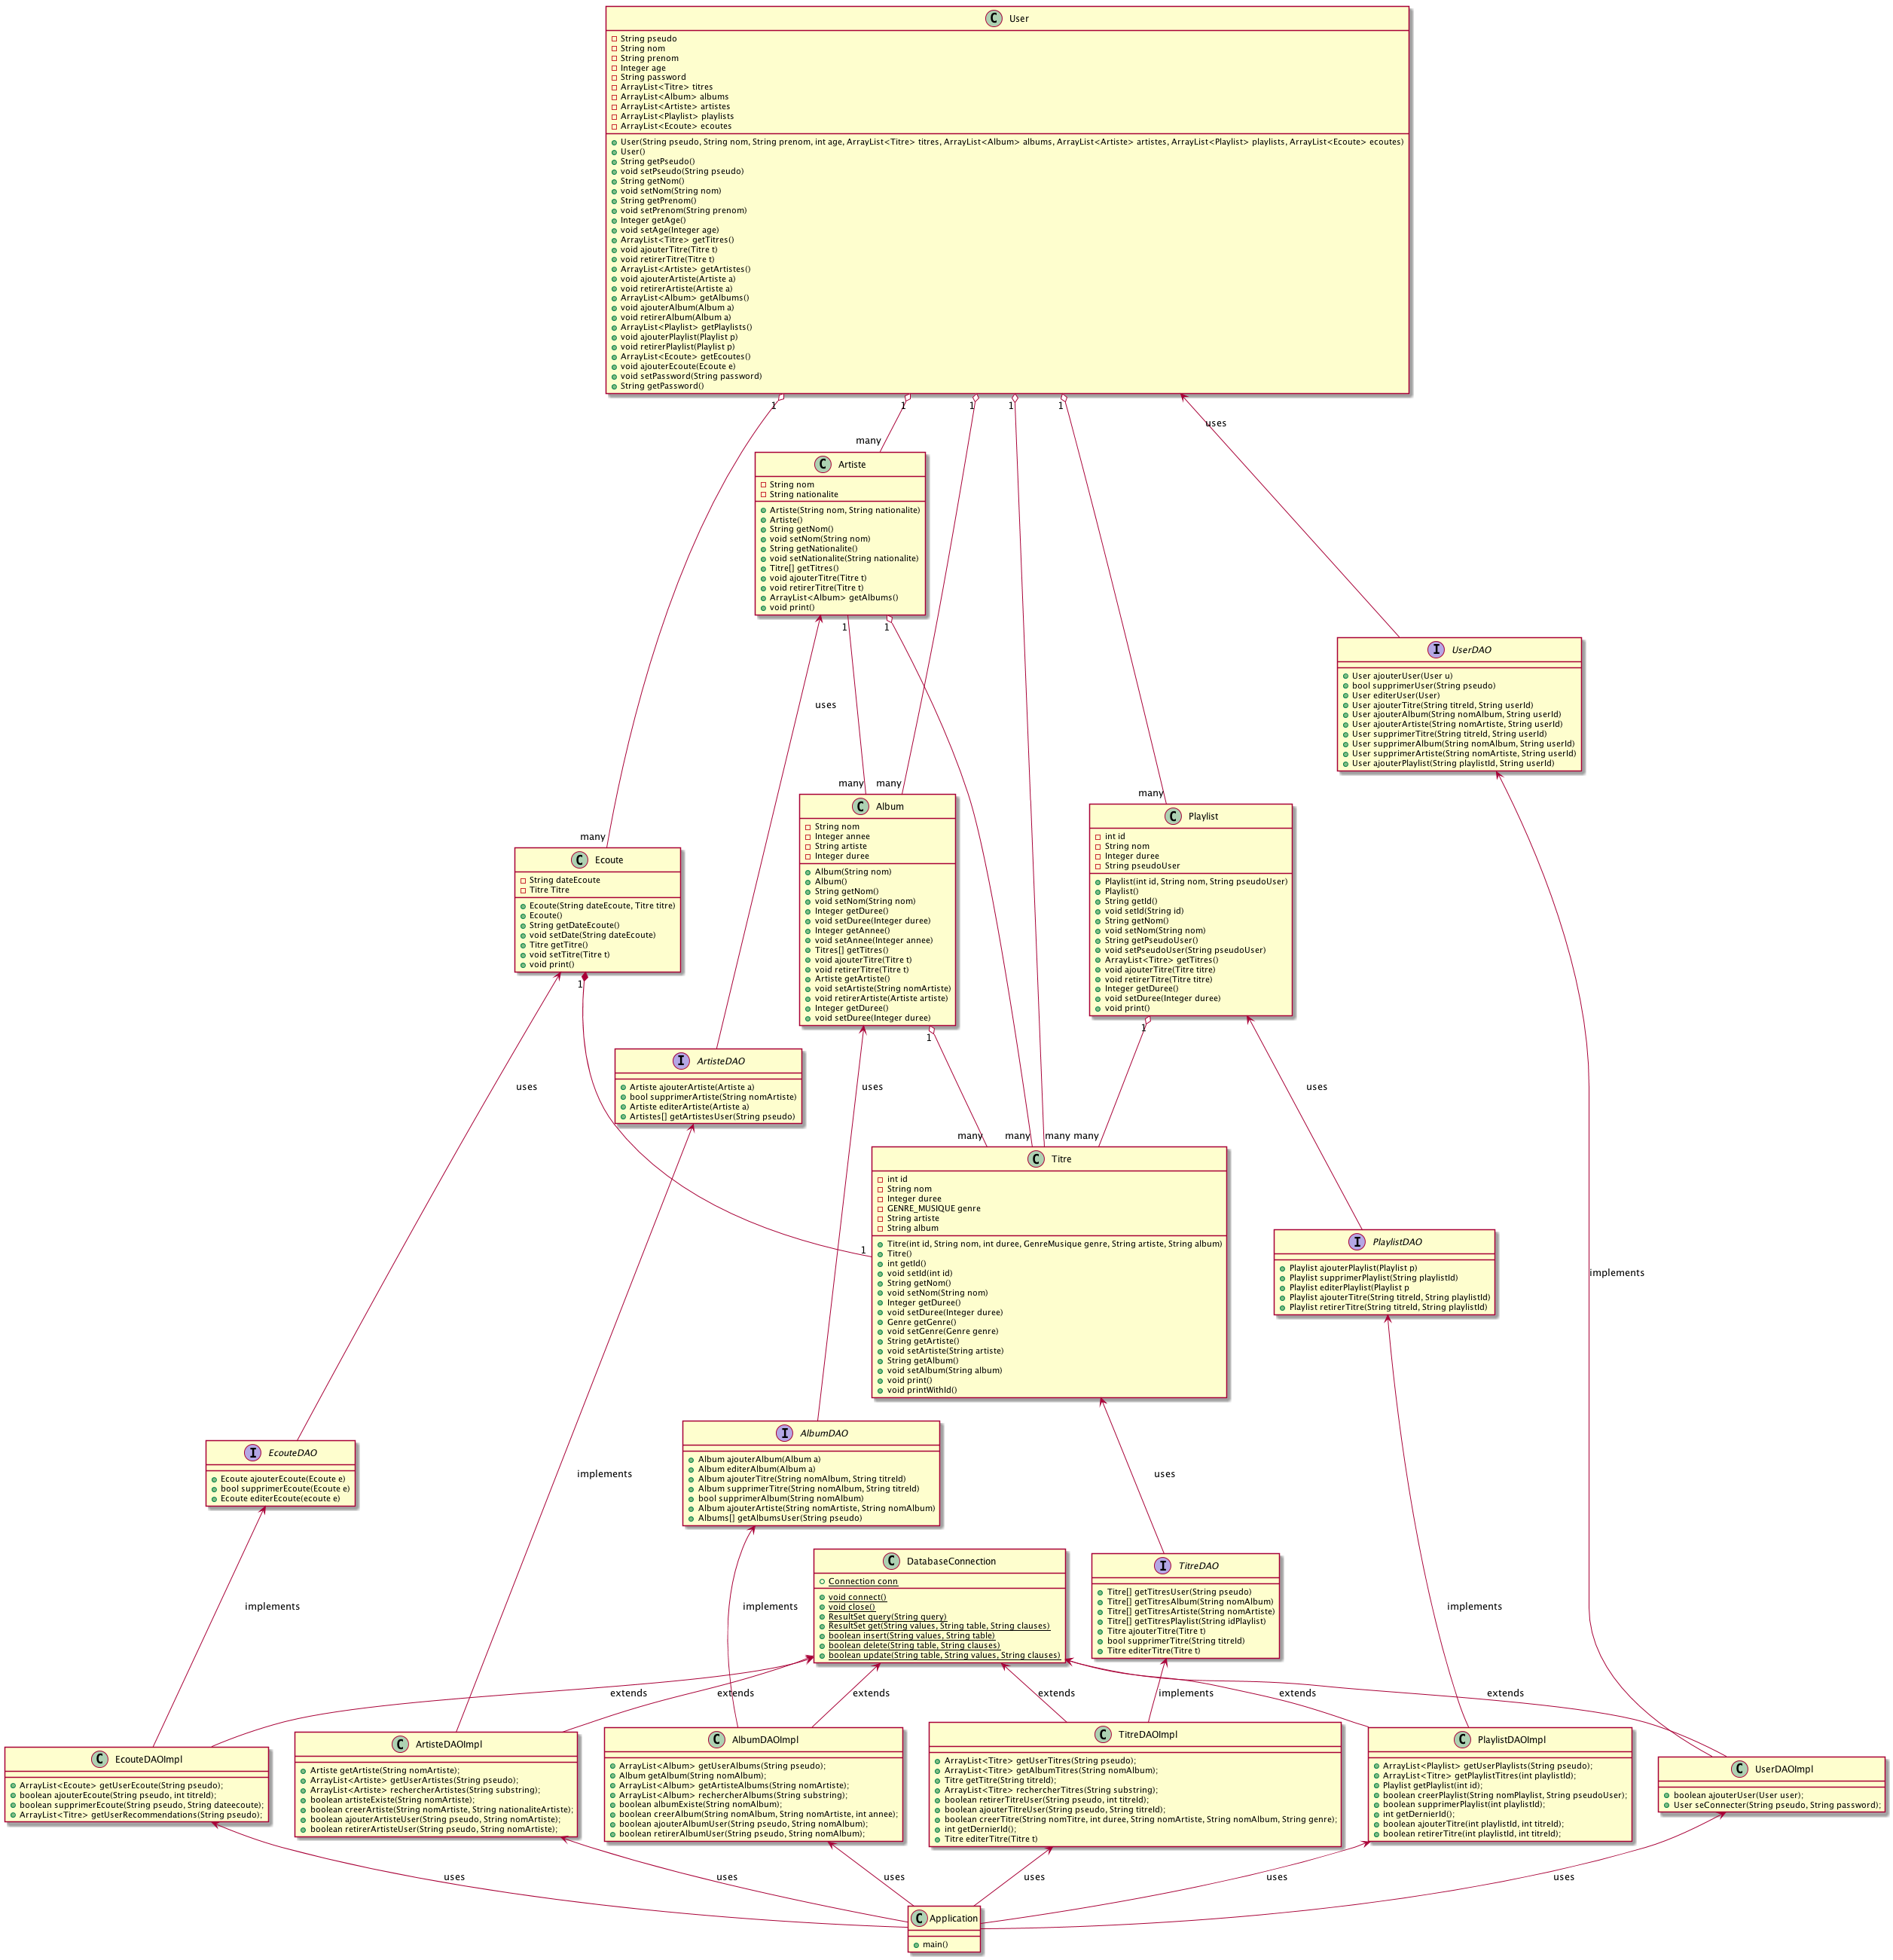
\includegraphics[scale=0.2]{class_diagram.png}
  \subsection{JDBC}
    Afin d'implémenter le design pattern \textbf{DAO}, nous allons utiliser \textbf{JDBC (Java Database Connectivity)}. JDBC est une \emph{API} pour JAVA permettant d'accéder à une base de donnée. Cette API fournit des méthodes pour se connecter à une base de données et effectuer des requêtes sur cette dernière depuis une application JAVA. L'utilisation de cette \emph{API} conjointement avec le design pattern \textbf{DAO} va se faire par l'intermédiaire d'une classe JAVA \textbf{DatabaseConnection} dont le rôle va être de créer une connexion à une base de donnée et d'implémenter les requêtes standard \textbf{select, update, insert, delete}. Cette classe va donc être une classe parente des implémentations des objets DAO.
\chapter*{Conclusion}


\end{document}
